\documentclass[12pt,a4paper]{article}
\usepackage[utf8]{inputenc}
\usepackage[T1]{fontenc}
\usepackage{geometry}
\usepackage{amsmath, amssymb}
\usepackage{listings}
\usepackage{xcolor}
\usepackage{booktabs}
\usepackage{array}
\usepackage{hyperref}
\usepackage{tikz}
\usetikzlibrary{graphs, positioning, arrows.meta}

\geometry{left=2.5cm, right=2.5cm, top=2.5cm, bottom=2.5cm}

\definecolor{codebg}{rgb}{0.96,0.96,0.96}
\definecolor{codegreen}{rgb}{0.0,0.5,0.0}
\definecolor{codegray}{rgb}{0.5,0.5,0.5}
\definecolor{codepurple}{rgb}{0.58,0,0.82}
\definecolor{codeblue}{rgb}{0.0,0.0,0.8}

\lstdefinestyle{javastyle}{
    backgroundcolor=\color{codebg},
    commentstyle=\color{codegreen}\itshape,
    keywordstyle=\color{codeblue}\bfseries,
    stringstyle=\color{codepurple},
    numberstyle=\tiny\color{codegray},
    basicstyle=\ttfamily\small,
    breaklines=true,
    keepspaces=true,
    numbers=left,
    numbersep=5pt,
    language=Java,
    frame=single,
    rulecolor=\color{codegray}
}

\hypersetup{colorlinks=true, linkcolor=blue, urlcolor=cyan}

\title{
    \Huge \textbf{Graph Traversal} \\[0.5em]
    \Large BFS \& DFS Algorithms \\[0.5em]
    \large Data Structures \& Algorithms Reference
}
\author{Algorithm Study Guide}
\date{\today}

\begin{document}

\maketitle
\tableofcontents
\newpage

% ============================================================
\section{Introduction to Graphs}
% ============================================================

A \textbf{graph} $G = (V, E)$ consists of a set of \textit{vertices} (nodes) $V$ and a set of \textit{edges} $E$ connecting pairs of vertices.

\subsection{Types of Graphs}
\begin{itemize}
    \item \textbf{Directed (Digraph)}: Edges have a direction $u \to v$.
    \item \textbf{Undirected}: Edges are bidirectional $u - v$.
    \item \textbf{Weighted}: Edges have a numerical weight.
    \item \textbf{Unweighted}: All edges are equal.
    \item \textbf{Cyclic / Acyclic}: Contains / doesn't contain cycles.
    \item \textbf{Connected}: Every vertex is reachable from every other vertex.
\end{itemize}

\subsection{Graph Representations}
\begin{enumerate}
    \item \textbf{Adjacency Matrix}: $V \times V$ boolean matrix. $O(V^2)$ space.
          Best for \textit{dense} graphs; quick edge lookup $O(1)$.
    \item \textbf{Adjacency List}: Array of lists. $O(V + E)$ space.
          Best for \textit{sparse} graphs; used in BFS and DFS.
\end{enumerate}

\subsection{Complexity Summary}
\begin{table}[h!]
\centering
\begin{tabular}{|l|c|c|}
\hline
\textbf{Algorithm} & \textbf{Time} & \textbf{Space} \\
\hline
BFS & $O(V + E)$ & $O(V)$ \\
DFS & $O(V + E)$ & $O(V)$ \\
\hline
\end{tabular}
\caption{$V$ = vertices, $E$ = edges}
\end{table}

\newpage

% ============================================================
\section{BFS — Breadth-First Search}
% ============================================================

\subsection{Concept}
BFS explores a graph \textbf{level by level}: starting from a source vertex, it visits all vertices at distance 1, then all at distance 2, and so on. It uses a \textbf{Queue} (FIFO) to maintain the traversal order.

\subsection{Algorithm}

\begin{enumerate}
    \item Mark source vertex $s$ as visited; enqueue $s$.
    \item While queue is not empty:
    \begin{enumerate}
        \item Dequeue vertex $u$ and process it.
        \item For each unvisited neighbor $v$ of $u$:
        \begin{itemize}
            \item Mark $v$ as visited.
            \item Enqueue $v$.
        \end{itemize}
    \end{enumerate}
\end{enumerate}

\subsection{Visual Example}

\begin{center}
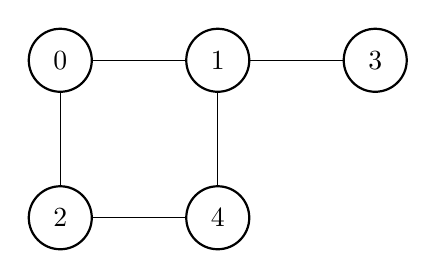
\begin{tikzpicture}[
    node distance=2cm,
    every node/.style={circle, draw, minimum size=0.8cm, thick},
    every edge/.style={draw, thick}
]
\node (0) {0};
\node (1) [right of=0] {1};
\node (2) [below of=0] {2};
\node (3) [right of=1] {3};
\node (4) [right of=2] {4};

\draw (0) -- (1);
\draw (0) -- (2);
\draw (1) -- (3);
\draw (1) -- (4);
\draw (2) -- (4);
\end{tikzpicture}
\end{center}

\textbf{BFS from vertex 0}:
\[
0 \xrightarrow{\text{Level 1}} 1, 2 \xrightarrow{\text{Level 2}} 3, 4
\]
\textbf{BFS order}: $0, 1, 2, 3, 4$

\subsection{Shortest Path Property}
BFS naturally finds the \textbf{shortest path} (minimum number of edges) in an \textbf{unweighted} graph. The distance array $d[v]$ stores the number of edges from source to $v$.
\[
d[v] = d[u] + 1 \quad \text{(when } v \text{ is first discovered from } u \text{)}
\]

\subsection{Java Implementation}
\begin{lstlisting}[style=javastyle, caption={BFS — Java}]
public void bfs(int start) {
    boolean[] visited = new boolean[vertices];
    Queue<Integer> queue = new LinkedList<>();
    visited[start] = true;
    queue.add(start);
    while (!queue.isEmpty()) {
        int node = queue.poll();
        System.out.print(node + " ");
        for (int neighbor : adjList.get(node)) {
            if (!visited[neighbor]) {
                visited[neighbor] = true;
                queue.add(neighbor);
            }
        }
    }
}
\end{lstlisting}

\subsection{Complexity}
\begin{itemize}
    \item \textbf{Time}: $O(V + E)$ — each vertex and edge visited once.
    \item \textbf{Space}: $O(V)$ — visited array + queue can hold up to $V$ vertices.
\end{itemize}

\subsection{Applications}
\begin{itemize}
    \item \textbf{Shortest path} in unweighted graphs.
    \item \textbf{Level-order} tree traversal.
    \item \textbf{Web crawlers}: explore links level by level.
    \item \textbf{Social networks}: find friends-of-friends (degrees of separation).
    \item \textbf{Bipartite graph checking}: color alternate levels differently.
    \item \textbf{GPS}: finding nearest location (e.g., nearest petrol station).
\end{itemize}

\newpage

% ============================================================
\section{DFS — Depth-First Search}
% ============================================================

\subsection{Concept}
DFS explores a graph by going as \textbf{deep as possible} along each branch before backtracking. It uses \textbf{recursion} (implicit call stack) or an explicit \textbf{Stack} (LIFO).

\subsection{Algorithm (Recursive)}

\begin{enumerate}
    \item Mark current vertex $u$ as visited and process it.
    \item For each unvisited neighbor $v$ of $u$: recursively call DFS($v$).
    \item \textbf{Backtrack} when all neighbors of $u$ are visited.
\end{enumerate}

\subsection{Visual Example}

Using the same graph:

\textbf{DFS from vertex 0}:
\[
0 \to 1 \to 3 \;\;(\text{backtrack}) \to 4 \;\;(\text{backtrack}) \to 2
\]
\textbf{DFS order}: $0, 1, 3, 4, 2$

\subsection{DFS Tree \& Edge Classification}
During DFS, edges are classified as:
\begin{itemize}
    \item \textbf{Tree edges}: edges in the DFS spanning tree.
    \item \textbf{Back edges}: connect a vertex to an ancestor (indicate a \textit{cycle}).
    \item \textbf{Forward/Cross edges}: occur in directed graphs.
\end{itemize}

\subsection{Java Implementation}
\begin{lstlisting}[style=javastyle, caption={DFS Recursive — Java}]
public void dfs(int node, boolean[] visited) {
    visited[node] = true;
    System.out.print(node + " ");
    for (int neighbor : adjList.get(node)) {
        if (!visited[neighbor]) {
            dfs(neighbor, visited);
        }
    }
}
\end{lstlisting}

\begin{lstlisting}[style=javastyle, caption={DFS Iterative (Stack) — Java}]
public void dfsIterative(int start) {
    boolean[] visited = new boolean[vertices];
    Deque<Integer> stack = new ArrayDeque<>();
    stack.push(start);
    while (!stack.isEmpty()) {
        int node = stack.pop();
        if (!visited[node]) {
            visited[node] = true;
            System.out.print(node + " ");
            for (int neighbor : adjList.get(node))
                if (!visited[neighbor]) stack.push(neighbor);
        }
    }
}
\end{lstlisting}

\subsection{Complexity}
\begin{itemize}
    \item \textbf{Time}: $O(V + E)$ — each vertex and edge visited once.
    \item \textbf{Space}: $O(V)$ for visited array + $O(h)$ for recursion stack ($h$ = max depth).
\end{itemize}

\subsection{Applications}
\begin{itemize}
    \item \textbf{Cycle detection} in directed and undirected graphs.
    \item \textbf{Topological sorting} of Directed Acyclic Graphs (DAGs).
    \item \textbf{Finding strongly connected components} (Tarjan's / Kosaraju's algorithms).
    \item \textbf{Maze solving}: explore all possible paths.
    \item \textbf{Detecting connectivity}: is the graph connected?
    \item \textbf{Solving puzzles}: Sudoku, N-Queens (backtracking).
\end{itemize}

\newpage

% ============================================================
\section{BFS vs DFS Comparison}
% ============================================================

\begin{table}[h!]
\centering
\renewcommand{\arraystretch}{1.5}
\begin{tabular}{|l|p{5.5cm}|p{5.5cm}|}
\hline
\textbf{Property}     & \textbf{BFS}                         & \textbf{DFS}                          \\
\hline
Data Structure        & Queue (FIFO)                          & Stack / Recursion (LIFO)              \\
Order                 & Level by level                        & Deep first, then backtrack            \\
Shortest Path         & \textbf{Yes} (unweighted graph)       & No                                    \\
Memory Usage          & Can be large (stores all frontier nodes) & Generally smaller (only current path) \\
Time Complexity       & $O(V+E)$                             & $O(V+E)$                             \\
Space Complexity      & $O(V)$                               & $O(V)$ visited + $O(h)$ stack         \\
Completeness          & Complete (finds shallowest solution)  & May get stuck in deep/infinite paths  \\
Best For              & Shortest path, level-order traversal  & Cycle detection, topological sort     \\
\hline
\end{tabular}
\caption{BFS vs DFS Comparison}
\end{table}

\section{Key Formulas}
\begin{align}
\text{BFS/DFS Time Complexity:}\quad & T(V,E) = O(V + E) \\
\text{BFS Shortest Distance:}\quad    & d[v] = d[u] + 1 \quad \forall \text{ edge } (u,v) \\
\text{Graph connected iff BFS/DFS visits all } V \text{ vertices.}
\end{align}

\end{document}
